\chapter{Few-shot object detection}
\label{chap:FSOD}
Il existe des cas de figures où le manque de données annotées pour un détecteur est poussé à l'extrême. On peut disposer, par exemple, que de moins de 5 images par catégorie d'objets à détecter. La few-shot object detection (FSOD) tente de régler la problématique liée à ce genre de configuration. Dans ce chapitre, nous donnons une formalisation de la FSOD et catégorisons les solutions proposées dans les articles de recherche. Nous explorons aussi les enjeux et les verrous scientifiques présents dans la problématique.


\section{Le few-shot meta-learning dans la classification d'images}
\label{sec:FSOD-FSL-meta}
La problématique que tente de résoudre le few-shot learning se pose aussi dans d'autres techniques de vision artificielle, notamment en classification d'images \cite{FSL-survey} où la communauté travaille sur le sujet depuis plus longtemps que pour la détection d'objets. Nous pensons qu'il est important de placer le contexte du few-shot learning en classification, étant donné que l'état de l'art dans cette technique influence grandement les travaux liés à la FSOD.

\subsection*{Formalisation du problème de few-shot classification}
On parle d'un problème de few-shot classification "$N$-way $K$-shot" pour qualifier le problème où l'on cherche à reconnaître des images de $N$ classes différentes. Pour chacune des $N$ classes, on dispose d'un nombre $K$ réduit d'images supervisées. Habituellement, un problème de few-shot classification se pose sur base d'un nombre d'images $K$ allant de 1 à 10.

\subsection*{Meta-learning en few-shot classification}
Récemment, de grands progrès ont été réalisés en few-shot learning pour la classification \cite{FSL-survey}. Ces progrès sont principalement dus à l'exploitation des méthodes de \textbf{meta-learning}.

Le meta-learning, aussi connu sous le nom de "learning to learn" \footnote{"Apprendre à apprendre", en français.}, est un paradigme qui consiste à faire apprendre à un réseau de neurones à s'adapter le plus rapidement possible à une tâche cible $\textbf{T}$ en se basant sur une "connaissance antérieure" apprise en tentant de résoudre plusieurs tâches d'entraînement $\{\textbf{T}_i\}$. Cette connaissance antérieure se veut assez générale pour permettre au réseau de neurones de s'adapter à des tâches différentes.

Concrètement, en classification d'images, $\textbf{T}$ correspond à la tâche $N$-way $K$-shot de classification d'images recherchée et les tâches $\{\textbf{T}_i\}$ sont d'autres problèmes $N$-way $K$-shot avec lesquelles le modèle apprend à s'adapter plus rapidement à une nouvelle tâche. Les données nécessaires aux tâches $\{\textbf{T}_i\}$ sont reprises de datasets déjà existant\footnote{COCO \cite{COCO}, ImageNet \cite{ILSVRC15}, etc.}. De ce fait, les images des datasets sont reprises, les seules images annotées qui doivent être manuellement produites pour résoudre le problème $N$-way $K$-shot sont celles nécessaires pour $\textbf{T}$.

Le paradigme du meta-learning prend forme de plusieurs manières différentes. Deux variantes nous intéresse pour la suite de ce chapitre :
\begin{itemize}
    \item \textbf{Basé sur le "metric learning"} \cite{prototypical-networks, matching-networks, koch2015siamese, relation-net-fsl} : le modèle réduit l'image en entrée en un vecteur de caractéristiques, d'une dimension inférieure à l'image de base. Ce vecteur est une métrique servant à calculer une distance entre d'autres vecteurs représentant d'autres images. Le modèle apprend donc à calculer une métrique dont la distance entre deux images d'une même classe est minimisée et la distance entre deux images de classes différentes est maximisée. On est alors capable de classer une image sur base de ces distances.
    \item \textbf{Optimisation des paramètres du réseau de neurones} \cite{MAML, Meta-SGD} : le modèle apprend, à l'aide des tâches d'entraînement $\{\textbf{T}_i\}$, à produire une bonne initialisation de ses paramètres (les poids, les meta-paramètres pour la fonction d'optimisation\footnote{Par exemple, le "learning rate" pour la descente de gradient.}, ...) d'une manière à ce qu'il puisse être performant pour résoudre $\textbf{T}$.
\end{itemize}

% Les enjeux
\section{Les enjeux}
\label{sec:FSOD-verrous}
Bien que l'importance de la problématique à laquelle tente de répondre la FSOD est avérée, il n'existe pas encore de méthode efficace et reconnue par la communauté. Ceci est dû aux raisons suivantes, qui sont détaillées dans cette section.

\subsection*{Domaine récent}
\label{subsec:domaine-recent}

La détection d'objets sur base du few-shot learning est un problème qui n'est abordé que depuis très récemment dans la communauté. À notre connaissance, les premiers travaux traitant du sujet ont commencé en 2018 avec \cite{feature-reweighting}. Ce caractère récent de la problématique implique les conséquences suivantes :
\begin{itemize}
    \item Peu d'articles de recherche ont été rédigés pour répondre au problème, ce qui implique qu'il y a encore un nombre de solutions limité à l'heure actuelle.
    \item Les solutions envisagées suivent, pour la majorité, une même tendance mais sont relativement hétérogènes dans leur procédé. Malgré cela, elles montrent des résultats similaires. Il y a encore une difficulté pour identifier une technique précise qui présenterait le meilleur intérêt.
\end{itemize}

\subsection*{Complexité de la détection par rapport à la classification}
\label{subsec:complexite-detection}
Comme évoqué dans la section \ref{sec:FSOD-FSL-meta}, les méthodes de few-shot meta learning en classification parviennent à atteindre des résultats intéressants constituant actuellement l'état de l'art en few-shot classification. Cependant, il est difficile d'appliquer directement les mêmes solutions de few-shot meta-learning en détection d'objets. La détection d'objets est une tâche bien plus complexe que la classification pour deux raisons :
\begin{itemize}
    \item La détection est une tâche qui ne cherche pas uniquement à reconnaître une image mais qui cherche aussi à \textit{localiser} un ou même plusieurs objets.
    \item Les objets à détecter dans une image se trouvent dans des environnements souvent encombrés (\textit{ex. : contenu d'une armoire}) et qui peuvent comporter d'autres objets qui ne sont pas recherchés. Les détecteurs entraînés avec peu de données ont tendance à être trompés par ces objets non-pertinents, qu'ils essaient d'interpréter comme des objets appartenant aux catégories ciblées. La partie du détecteur posant problème est celle qui identifie les zones d'intérêt où pourraient se trouver potentiellement un objet recherché. 
\end{itemize}

La littérature traitant de la FSOD travaille essentiellement sur l'adaptation de ces variantes de meta-learning pour résoudre les soucis liés à la détection.

% Définition problème
\section{Formalisation du problème de FSOD}
\label{sec:FSOD-def-prob}
Dans cette section, nous décrivons de manière formelle le problème rencontré que tente de résoudre un algorithme de FSOD.

On parle de détection d'objets "$N$-way $K$-shot" pour qualifier le problème où le but est d'entraîner un détecteur $\phi$ pour que celui-ci soit capable de détecter dans une image des objets appartenant à $N$ catégories différentes. Pour chacune des $N$ catégories, nous disposons d'un nombre de $K$ images annotées, relativement réduit. Habituellement, un problème de FSOD se pose sur base d'un nombre d'images $K$ allant de 1 à 10. Il faut noter que, dans une même image, il peut y avoir plusieurs fois le même objet ou des objets de plusieurs des $N$ catégories en même temps. Ainsi, il est garanti qu'il existe au moins $K$ instances de chacune des $N$ catégories d'objets dans les données dont on dispose.

Pour régler ce problème, les solutions mises au point partent toutes d'une configuration commune : nous disposons de deux datasets : $D_{support}$ et $D_{query}$. $D_{support}$ comprend un grand nombre d'images déjà labélisées selon un ensemble de classes d'objets $C_{support}$, tandis que $D_{query}$ est composé de peu d'images annotées avec les classes $C_{query}$. En pratique, $D_{support}$ est un dataset déjà existant que l'on divise en tâches d'entraînement $\{\textbf{T}_i\}$ qui correspondent à plusieurs problèmes $N$-way $K$-shot. Les tâches $\{\textbf{T}_i\}$ servent à créer la connaissance antérieure du détecteur, qui sera alors capable de s'adapter pour améliorer sa détection sur la tâche cible $\textbf{T}$. $\textbf{T}$ est le problème $N$-way $K$-shot que le détecteur doit résoudre où les $K$ classes d'objets forment l'ensemble de classe $C_{query}$ et les $N \times K$ images labélisées forment $D_{query}$. La figure \ref{fig:Formalisation-FSOD} illustre cette configuration.

La phase d'apprentissage du détecteur est réalisée grâce aux tâches $\{\textbf{T}_i\}$. Ensuite, le détecteur est optimisé pour $\textbf{T}$ avec les $N \times K$ images disponibles pour $D_{query}$.
\begin{figure}[!h]
\centering
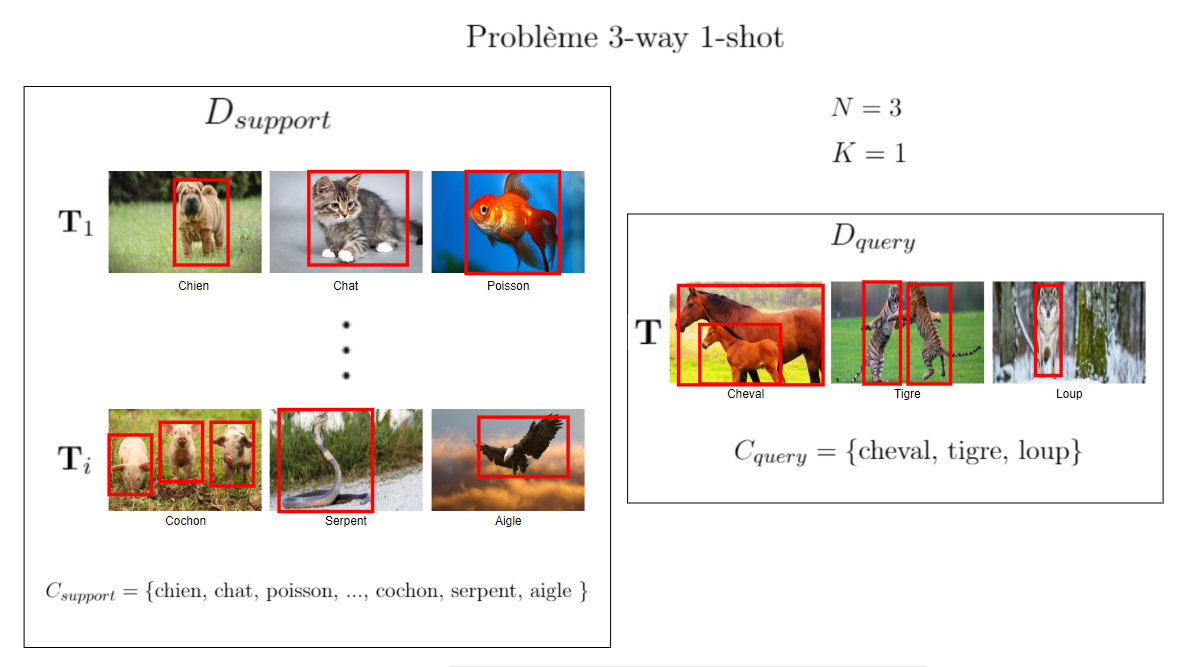
\includegraphics[scale=0.5]{img/Formalisation-FSOD.PNG}
\caption{Exemple de formalisation pour un problème 3-way 1-shot où le but est de détecter des chevaux, tigres et loups en utilisant un dataset de support d'animaux.}
\label{fig:Formalisation-FSOD}
\end{figure}

% Catégorisation solutions
\section{Catégorisation des solutions}
\label{sec:FSOD-categorisation}
Au vu du caractère récent de la recherche sur la FSOD, une catégorisation n'a pas encore été installée dans la communauté. On peut cependant constater qu'il n'existe, pour le moment, que des solutions utilisant le paradigme du meta-learning en FSOD. C'est pourquoi nous faisons le parallèle avec les variantes du paradigme de meta-learning utilisées en few-shot classification\footnote{Voir la section \ref{sec:FSOD-FSL-meta}.} pour définir une séparation plus claire pour la détection.

\subsection{Basé sur le metric learning}
Cette catégorie est la plus populaire à l'heure actuelle. Comme pour la classification, un détecteur basé sur du metric learning va calculer pour chaque image une représentation réduite d'image en vecteur de caractéristiques entre lesquelles on peut calculer une distance. Dans le cas de la détection, ce calcul d'une représentation est faite dans deux buts :
\begin{itemize}
    \item Discriminer les ROI trouvées par le détecteur afin de ne pas être trompé par les objets non-pertinents.
    \item Classifier les ROI restantes selon les $N$ catégories d'objets recherchées.
\end{itemize}

\subsubsection*{Vue d'ensemble de l'architecture}
On entraîne le détecteur sur les tâches $\{\textbf{T}_i\}$. Une tâche $\textbf{T}_i$ est composée de :
\begin{itemize}
    \item $\textbf{S}_i$ : un ensemble de $K$ images de support pour chacune des $N$ catégories que $\textbf{T}_i$ cherche à détecter. On dispose des localisations des objets dans ces images.
    \item $\textbf{V}_i$ : un ensemble de $Q$ images de validation. Une image de validation sert à évaluer la performance du détecteur pour la tâche, c'est-à-dire qu'on mesure la précision des bounding boxes trouvées par le détecteur par rapport à la vérité terrain. Cette évaluation de la détection sera ensuite utilisée pour améliorer les paramètres du réseau pour la prochaine tâche.
\end{itemize}

Le détecteur calcule, pour chaque classe, les vecteurs de caractéristiques sur base des objets localisés dans les images de $\textbf{S}_i$. Ces vecteurs prennent en compte la localisation des objets, afin de pouvoir ensuite discriminer les zones d'intérêt trouvées dans une image de validation.

\begin{figure}[!h]
\centering
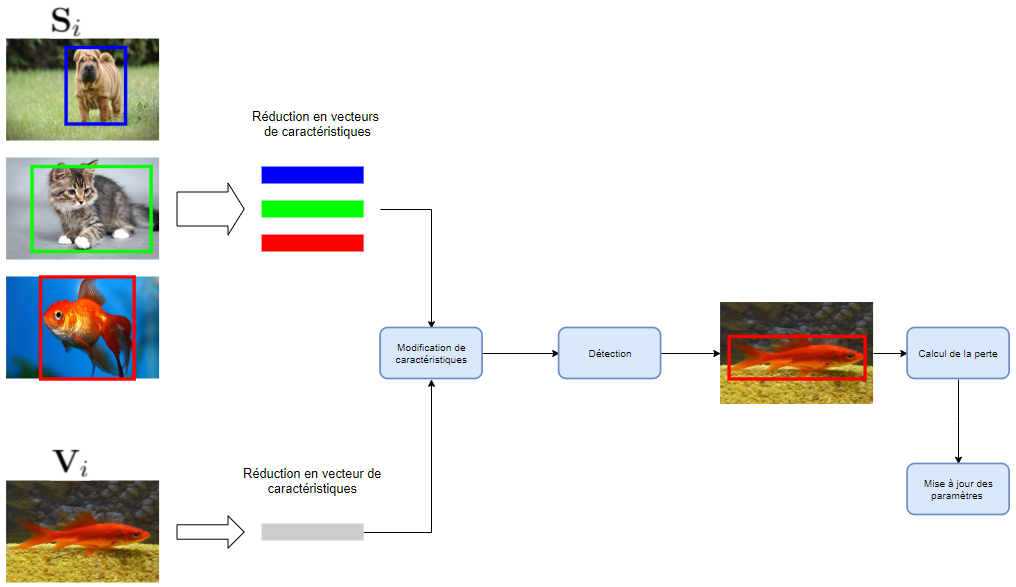
\includegraphics[scale=0.5]{img/DML.PNG}
\caption{Exemple d'entraînement pour une tâche $\textbf{T}_i$ de type 3-way 1-shot avec une seule image de validation pour $\textbf{V}_i$.}
\label{fig:DML}
\end{figure}

Après le calcul des vecteurs de caractéristiques de $\textbf{S}_i$, on évalue la détection grâce aux images de $\textbf{V}_i$. Pour chaque image de $\textbf{V}_i$, on calcule son vecteur des caractéristiques. On modifie celui-ci à l'aide des vecteurs des images de support avec une opération\footnote{Cette "opération" change fortement en fonction des articles. C'est pourquoi nous ne cherchons pas à la détailler ici.} dont le but est d'atténuer les caractéristiques de l'image de validation qui ne sont pas pertinentes et de "surligner" celles qui ont de l'importance par rapport aux objets recherchés. Ensuite, on applique un algorithme de détection propre à la méthode\footnote{Une variante de Faster R-CNN \cite{Faster-R-CNN}, SSD \cite{SSD}, YOLO \cite{YOLO}, etc. Tout dépend de l'algorithme de FSOD utilisé.} avec l'aide du vecteur de caractéristiques modifié par les vecteurs de $\textbf{S}_i$. On calcule ensuite la perte sur les détections trouvées pour l'image de $\textbf{V}_i$. On ré-entraîne l'entièreté du modèle (calcul des vecteurs de caractéristiques, détection, etc) sur base de cette perte. La figure \ref{fig:DML} illustre un résumé de la variante.

Après cette phase d'entraînement, le détecteur est capable de résoudre la tâche cible $\textbf{T}$. Il calcule les vecteurs de caractéristiques pour les $N\times K$ images de la tâche $\textbf{T}$ et est capable d'effectuer une détection pour $\textbf{T}$.


\subsection{Optimisation des paramètres du détecteur}
Cette pratique est moins développée que celle sur le metric-learning, c'est pourquoi nous choisissons de ne pas entrer dans les détails des explications ici. Le but de cette variante est de faire apprendre une optimisation de paramètres au détecteur, qui lui permettra de minimiser la perte le plus rapidement possible pour une nouvelle tâche. 

Les algorithmes de cette catégorie sont habituellement composés de deux composants : le détecteur et le \textit{meta-learner}. Le détecteur a pour rôle de réaliser une détection pour une tâche $\textbf{T}_i$. Le rôle du meta-learner est de créer une bonne adaptation des paramètres de ce détecteur afin que celui-ci soit capable de faire une meilleure détection pour la prochaine tâche.

Lors de l'entraînement, le détecteur apprend en résolvant une tâche $\textbf{T}_i$. Après l'opération de détection, le meta-learner calcule les "meta-info" sur base de la détection faite par le détecteur sur $\textbf{T}_i$. Ces meta-infos servent à faire apprendre au meta-learner à adapter les paramètres $\theta$ du détecteur ainsi que ses meta-paramètres. Pour la tâche suivante $\textbf{T}_{i+1}$, le meta-learner fournit les paramètres $\theta$ et les méta-paramètres optimisés au détecteur afin que celui-ci exécute une meilleure détection.

\hspace{1pt}
\par\noindent\rule{\textwidth}{0.4pt}

Comme nous l'expliquons dans ce chapitre, la FSOD est une problématique récente pour laquelle on recherche encore une solution qui s'impose par rapport aux autres. Nous montrons que le paradigme du meta-learning est actuellement une piste fortement exploitée pour y parvenir et qu'une de ses variantes, le metric learning, semble être la tendance la plus populaire. Les recherches en FSOD ayant débuté récemment, il n'existe pas encore de comparaison entre les algorithmes existants. Nous tentons donc, dans le chapitre \ref{chap:analyse}, de réaliser une comparaison des résultats publiés dans les articles de recherche.